\documentclass[12pt,a4paper]{article}
\synctex=1
\usepackage[utf8]{inputenc}
\usepackage[margin=1cm,bottom=2cm]{geometry}
\usepackage{graphicx}
%\usepackage{verbatim}
\usepackage{listings}
\usepackage{multicol}
\usepackage{libertine}
\usepackage{pgfornament}
\usepackage{eso-pic}
\usepackage{textcomp}
\usepackage{courier}
\usepackage[hangul]{kotex}
\linespread{1.3}

\title{
	\centering
	\pgfornament[width=12cm,color=teal]{84}\\
	\vspace{1cm}
	\fontsize{50}{50} \selectfont {동국 SW 공모대전\\SIC emulator 설명서}\\
	\pgfornament[width=12cm,color=teal]{88}\\
	\vfill}
\author{
	\LARGE
	\begin{tabular}{rl}
		\hline
		학번 : & 2016110056\\ 
		학과 : & 불교학부 \\
		이름 : & 박승원\\
		날짜 : & \today\\
		\hline
	\end{tabular}\vspace{2cm}
	\\
	\includegraphics[width=0.5\textwidth]{/home/zezeon/Dropbox/Photos/logo.jpg}
}
\date{}


\begin{document}
\maketitle
\newpage
\noindent
\lstset{columns=flexible, tabsize=4, frame=single, showstringspaces=false, breaklines=true, upquote=true}

\pagenumbering{gobble}
\lstset{language=C++}
\lstinputlisting[caption={1.s : Hello World in SIC}]{1.s}
\lstinputlisting[caption={2.s : X 레지스터의 값을 1 증가시키는 모듈}]{2.s}
\lstinputlisting[caption={1.s가 전처리된 소스 파일}]{/tmp/1.s}
\lstinputlisting[caption={2.s가 전처리된 소스 파일}]{/tmp/2.s}
\lstinputlisting[caption={1.o : 오브젝트 파일}]{1.o}
\lstinputlisting[caption={2.o : 오브젝트 파일}]{2.o}
\lstinputlisting[caption={1.x : 1.o와 2.o가 링크된 실행 파일}]{1.x}
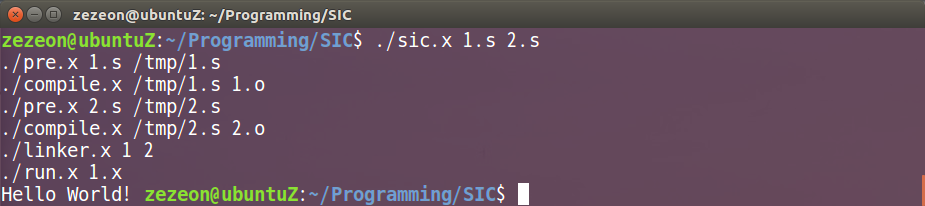
\includegraphics[width=\textwidth]{hello.png}
%\begin{multicols}{2}
2. 다음에 주어진 파일 입출력 프로그램을 참고하여 SIC srcfile을 assemble 할 때 출력되는 OBJFILE을 읽어서 각 줄의 TAG(첫 글자)가 'T'인 줄을 TAG, ADDR, LENGTH, CODES로 분리하고, 분리된 것 중에서 CODES에 해당하는 내용을 메모리 내부표현(internal representation)으로 변화(Code conversion)하고, 문자코드로 표현된 CODES와 코드변환된 InCodes(각 문자를 변환하여 10진법 표기 값)을 출력하는 프로그램을 구현하고 실습하시오.

\vspace{1cm}


{\Huge소감}
\indent
스트림 클래스가 유용했다. 

\end{document}
